\documentclass{article}

\usepackage{fullpage}
\usepackage{times}
\usepackage[pdftex]{graphicx}

\begin{document}

\parindent 0cm
\parskip 0.3cm

\title{Tiny Application Sensor Kit (TASK) Field Tool User Manual}
\author{David Gay, Intel Research \\
dgay@intel-research.net}
\date{March 19, 2003}
\maketitle

\section{Introduction}

The field tool is a simple tool for debugging TASK-based sensor networks
``in the field''. The field tool allows a user to walk up to a TASK-mote and
inspect or modify its state by issuing a set of simple commands. The field
tool only operates on the motes that are in direct radio range (i.e., close
proximity) to the user.

The field tool runs on handhelds devices (currently HP Ipaq's running Linux)
equipped with a {\tt Canby} or {\tt Canby2} compact-flash mote.

\section{Mode of Operation}

Before the first use, the field tool should be configured as explained
in Section~\ref{sec:config}.

Once started, the field tool presents the user with the screen shown in
Figure~\ref{fig:toolview}. The top-left pane is a list of commands
(``command pane'') that can be sent to the mote, the top-right pane is a
list of the motes (``mote pane'') that the field tool has discovered in the
local neighbourhood, the bottom pane (``result pane'') displays the results
returned of field tool commands as returned by the motes.

\begin{figure}[t]
\begin{center}
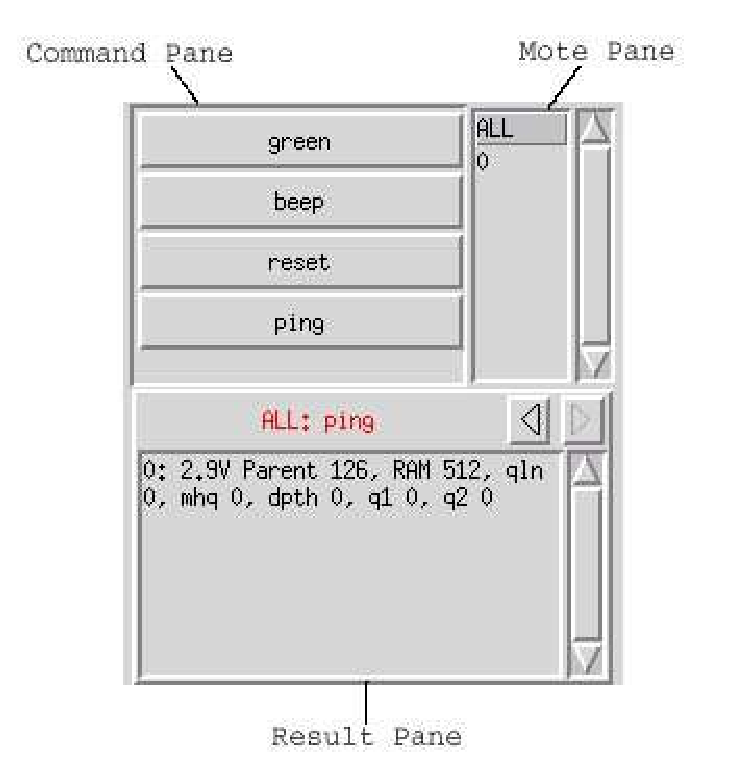
\includegraphics[width=3in]{./fig/fieldtool-gui.pdf}
\end{center}
\caption{Field Tool User Interface.}
\label{fig:toolview}
\end{figure}

TASK-motes spend most of their time asleep; they will not discover (and be
discovered by) the field tool until the next time they wake up. Once a mote
notices the field tool, it will turn on its yellow LED\footnote{{\tt
mica2dot} motes do not have yellow LEDs, so you won't see anything.} and
switch to an ``always-on'' state. Simultaneously, assuming no radio
problems, the field tool will update the list of motes known to be in the
neighbourhood (top-right pane).

The field tool advertises its presence by sending periodic messages. The
interval between these periodic messages can be changed with the field tool
configurator (Section~\ref{sec:config}). If a mote does not hear from the
field tool for 20s, it assumes that it can return to normal operation,
turns off its yellow LED, and resumes its regular sleep/wake
schedule. Similarly, if the field tool does not hear from a mote for 10s
(or the ``Mote Timeout'' value chosen using the configurator), it assumes
that the mote is no longer in proximity to the field tool and removes it
from the mote list in the top-right pane.

Sending commands to motes is straightforward:
\begin{enumerate}
\item Select a specific mote from the mote list, or select ``ALL'' to send
a command to all motes in the range of the field tool (which should be 
the same as those shown in the mote list).
\item Execute the desired command by clicking on its button in the top-left
command pane.
\end{enumerate}
The results of the command, as returned by the motes, are shown in the
result (bottom) pane. Results are of the form ``mote number: command
results'', with one entry per mote that received the command. Note that
problems with radio connectivity may lead the mote to execute the command,
but prevent the mote's answer from being displayed by the field tool.

It is possible to scroll through the answers from previous commands using
the left and right arrows at the top-right of the result pane. The title
area of the result pane shows the destination of the command (ALL or a mote
number), the command name and the time the command was executed. The
results from the latest command are displayed in red, without a time.

\section{Field Tool Commands}

There are currently four commands defined in the field tool:
\begin{itemize}
\item {\bf green}: toggle the green LED.\footnote{{\tt mica2dot} motes
do not have green LEDs, so you won't see anything, but you will still
get the ``done'' result.}
This can be used to check that
field tool/mote communication is working. Motes just return ``done'' as the
result.
\item {\bf beep}: sound the mote's sounder -- this obviously requires the
standard mica sensor board. The purpose is similar to
``green''. Motes just return ``done'' as the result.
\item {\bf reset}: Reset the mote. Note: this command has no result (as the
mote just reset itself...).
\item {\bf ping}: Return vital statistics on the operation of the TASK-mote.
The result is of the form ``X V, Parent N, RAM R, qln Q, mhq M, dpth D, qual L, q1 Q1, q2 Q2'', where:
\begin{itemize}
\item X is the current voltage of the mote's batteries.
\item N is the parent of this mote in the routing tree.
\item R is the amount of RAM available for queries on this mote.
\item Q is the radio send queue length.
\item M is the forward queue length of the multi-hop routing layer.
\item D is the depth of the mote in the multi-hop routing tree, i.e., the number
of hops to root.
\item L is the link quality of the current parent node.  The metric is routing layer-dependent.
\item Q1 is the query id of the first TinyDB query currently running, typically the TASK sensor query.  $-1$ means no query.
\item Q2 is the query id of the second TinyDB query currently running,
typically the TASK health query.  $-1$ means no second query.
\end{itemize}
\end{itemize}

\section{Field Tool Configuration}
\label{sec:config}

The Canby mote should be programmed with the {\tt GenericBase} application,
programmed with
\begin{verbatim}
  make <motekind> -DCANBY MSG_SIZE=49
\end{verbatim}
where {\tt <motekind>} is {\tt mica} or {\tt mica2}. On {\tt mica2}s and
{\tt mica2dot}s, if you're not using the default 433MHz channel, you should
make sure that you have selected the correct radio frequency either in
your Makelocal file, or via {\tt -DCC1K\_DEF\_FREQ=<DesiredFreq>} or {\tt
-DCC1K\_DEF\_PRESET=<Index>} {\tt ncc} options.


\begin{figure}[t]
\begin{center}
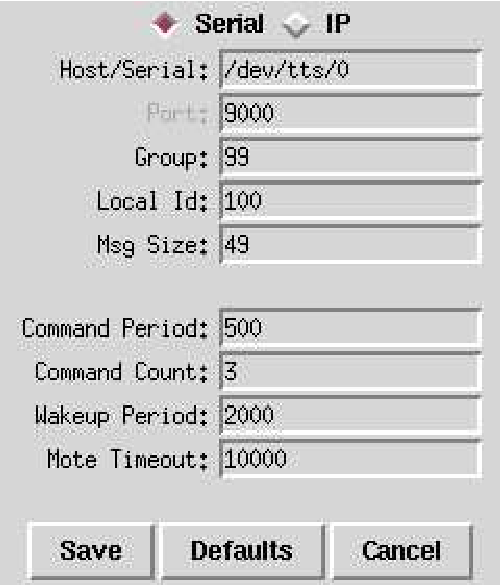
\includegraphics[width=2.2in]{./fig/fieldtool-config.pdf}
\end{center}
\caption{Field Tool Configurator.}
\label{fig:configview}
\end{figure}

The field tool configurator must be used to set up important field tool
parameters. The interface of this configurator is shown in Figure~\ref{fig:configview}. The following parameters can be set:
\begin{itemize}
\item {\bf Serial or IP}: choose whether the field tool communicates with
the Canby mote (or equivalent) over IP or via a serial port. This should
normally be left at ``Serial''.

\item {\bf Host/Serial}: Hostname for IP communication when IP is chosen,
serial port name when Serial is chosen. Normally ``/dev/tts/0''.

\item {\bf Port/Baud}: Portname for IP communication, baud rate for serial
communications (mica-based Canby motes use 19200 baud, mica2-based Canby
motes use 57600 baud).

\item {\bf Group}: group id of the TASK motes. You must set this to match
the group ID of your generic sensor kit deployment. Also, the Canby mote
must be programmed with this group ID.

\item {\bf Local Id}: ID for the field tool. Should be different from
any TASK-mote ID.

\item {\bf Msg Size}: Mote radio message size. Must be 56.

\item {\bf Command Period}: the commands selected by the user are sent
multiple times to ensure reception by the motes. This value is the interval 
in ms at which messages are repeated. Normally 500ms.

\item {\bf Command Count}: the number of times commands selected by the user
are sent. Normally 3.

\item {\bf Wakeup Period}: the interval (in ms) between the messages the
field tool sends to advertise its presence to motes. Must be smaller than
half the normal awake period of the motes, or they will not notice the
field tool.

\item {\bf Mote Timeout}: interval (in ms) after which motes which have not
been heard by the field tool are removed from the mote list. Default is 10s.
This should be at least twice the wakeup period to avoid motes constantly
appearing and disappearing from the mote list.

\end{itemize}

\end{document}
% LocalWords:  TASK handhelds Ipaq's Canby neighbourhood configurator qln mhq IP
% LocalWords:  dpth Hostname Msg
